\documentclass{standalone}
\usepackage{tikz}
\usetikzlibrary{patterns, positioning}
\usepackage[sfdefault]{ClearSans} %% option 'sfdefault' activates Clear Sans as the default text font
\usepackage[T1]{fontenc}

\begin{document}
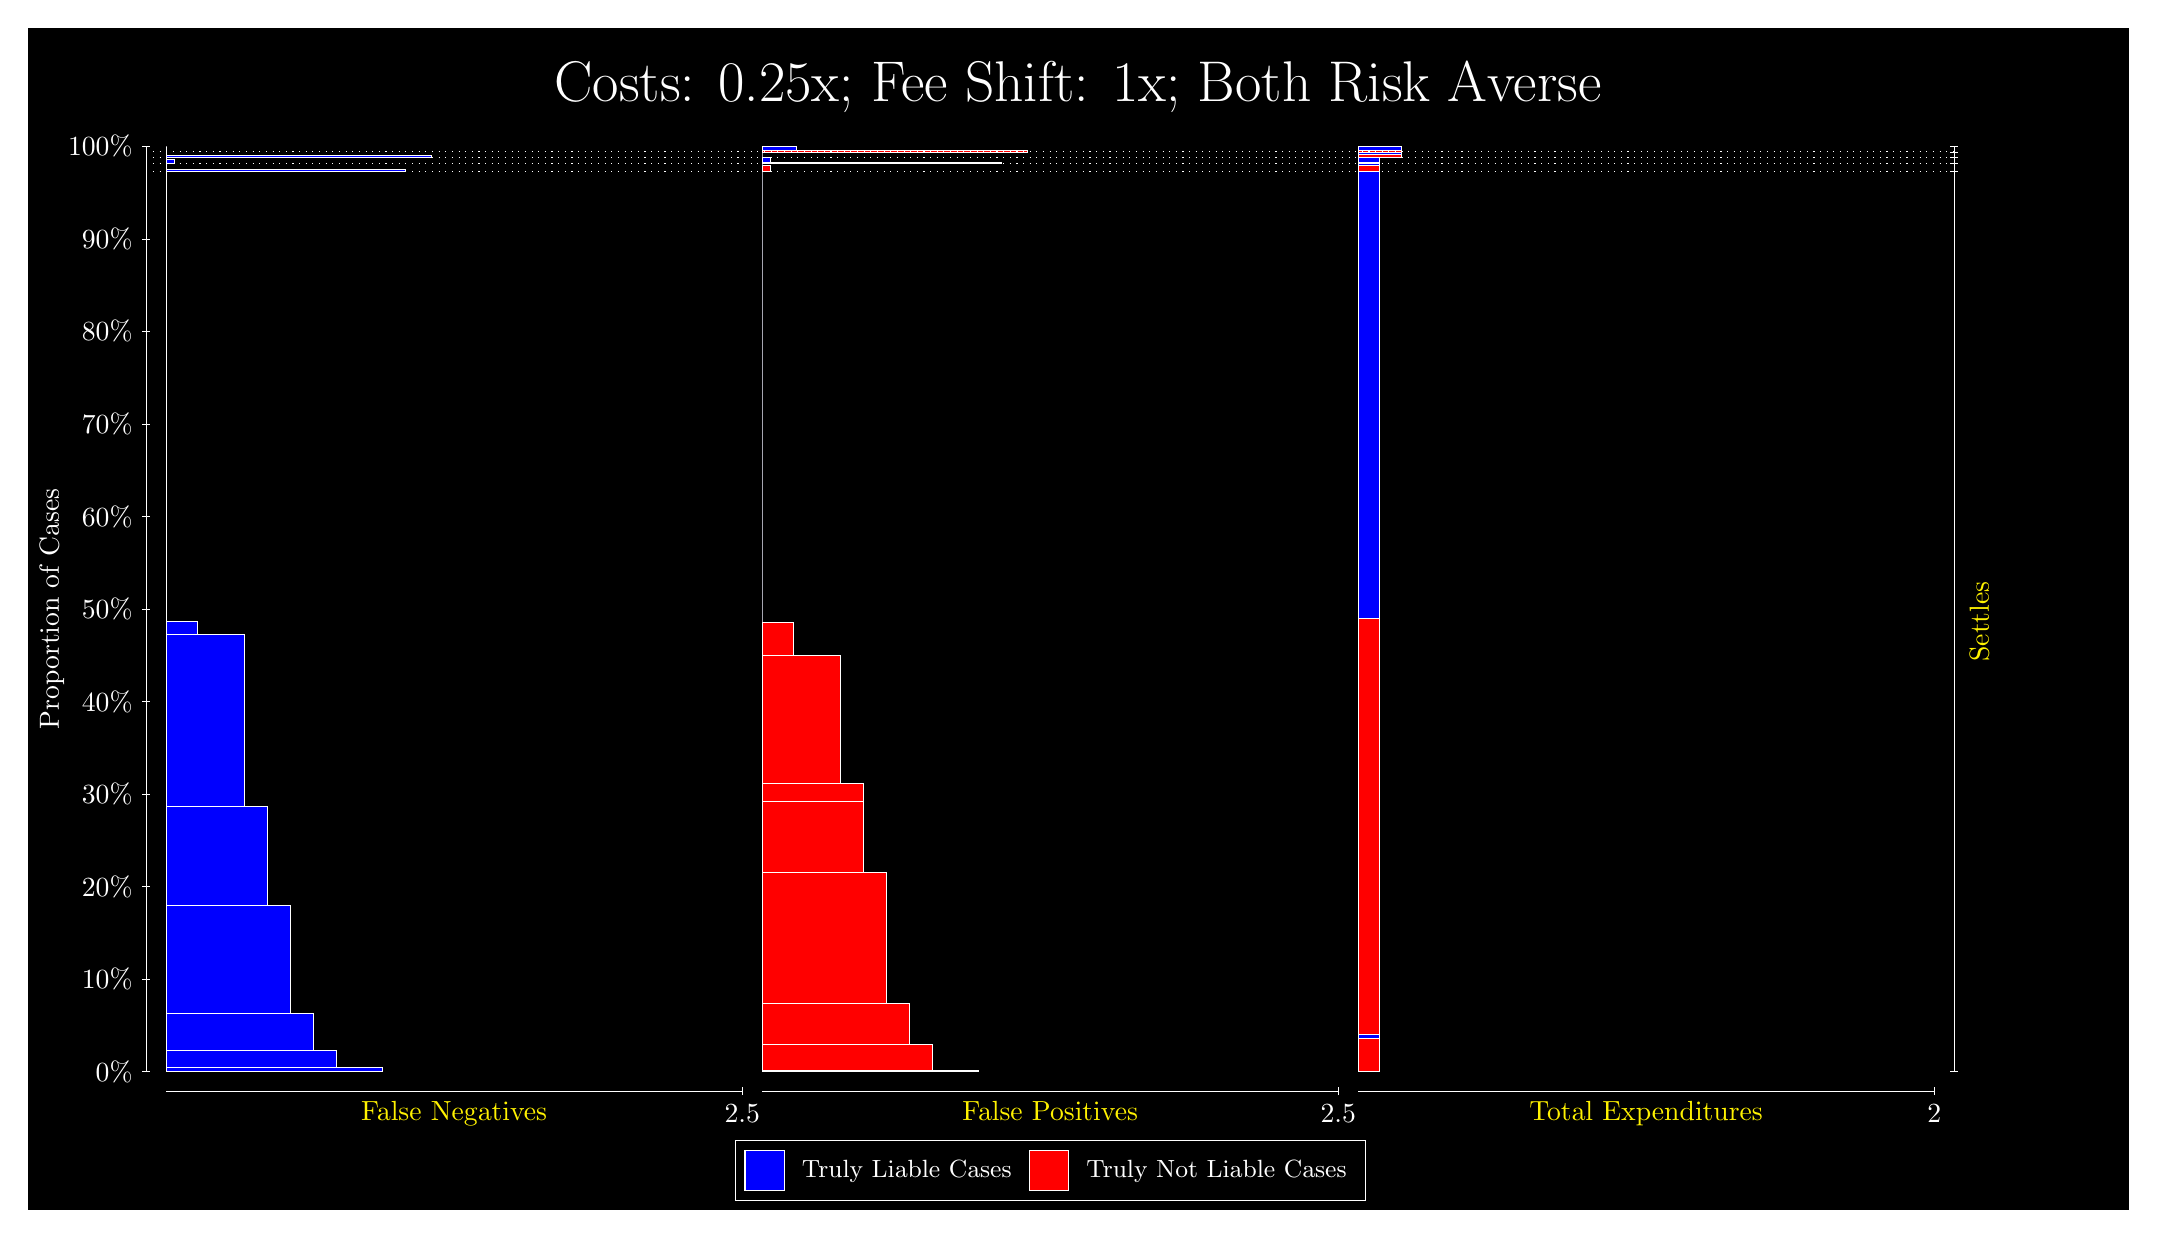
\begin{tikzpicture}
\draw[fill=black] (0,0) rectangle (26.667,15);
\draw[text=white] (0,13.5) rectangle (26.667,15) node[midway] {\huge Costs: 0.25x; Fee Shift: 1x; Both Risk Averse};
\draw[white, very thin] (1.5,1.75) -- (1.5,13.5);
\node[rotate=90, text=white, anchor=center] at (0.3, 7.625) {Proportion of Cases};
\draw[white, very thin] (1.45,1.75) -- (1.55,1.75);
\node[text=white, anchor=east] at (1.45, 1.75) {0\%};
\draw[white, very thin] (1.45,2.925) -- (1.55,2.925);
\node[text=white, anchor=east] at (1.45, 2.925) {10\%};
\draw[white, very thin] (1.45,4.1) -- (1.55,4.1);
\node[text=white, anchor=east] at (1.45, 4.1) {20\%};
\draw[white, very thin] (1.45,5.275) -- (1.55,5.275);
\node[text=white, anchor=east] at (1.45, 5.275) {30\%};
\draw[white, very thin] (1.45,6.45) -- (1.55,6.45);
\node[text=white, anchor=east] at (1.45, 6.45) {40\%};
\draw[white, very thin] (1.45,7.625) -- (1.55,7.625);
\node[text=white, anchor=east] at (1.45, 7.625) {50\%};
\draw[white, very thin] (1.45,8.8) -- (1.55,8.8);
\node[text=white, anchor=east] at (1.45, 8.8) {60\%};
\draw[white, very thin] (1.45,9.975) -- (1.55,9.975);
\node[text=white, anchor=east] at (1.45, 9.975) {70\%};
\draw[white, very thin] (1.45,11.15) -- (1.55,11.15);
\node[text=white, anchor=east] at (1.45, 11.15) {80\%};
\draw[white, very thin] (1.45,12.325) -- (1.55,12.325);
\node[text=white, anchor=east] at (1.45, 12.325) {90\%};
\draw[white, very thin] (1.45,13.5) -- (1.55,13.5);
\node[text=white, anchor=east] at (1.45, 13.5) {100\%};

\draw[white, very thin] (24.457,1.75) -- (24.457,13.5);
\draw[white, very thin] (24.407,1.75) -- (24.507,1.75);
\node[anchor=west] at (24.407, 1.75) {};
\draw[white, very thin] (24.407,13.182) -- (24.507,13.182);
\node[anchor=west] at (24.407, 13.182) {};
\draw[white, very thin] (24.407,13.28) -- (24.507,13.28);
\node[anchor=west] at (24.407, 13.28) {};
\draw[white, very thin] (24.407,13.358) -- (24.507,13.358);
\node[anchor=west] at (24.407, 13.358) {};
\draw[white, very thin] (24.407,13.43) -- (24.507,13.43);
\node[anchor=west] at (24.407, 13.43) {};
\draw[white, very thin] (24.407,13.5) -- (24.507,13.5);
\node[anchor=west] at (24.407, 13.5) {};

\draw[white, very thin, fill=blue] (1.75,1.75) rectangle (4.4946,1.8008);
\draw[white, very thin, fill=blue] (1.75,1.8008) rectangle (3.9091,2.0196);
\draw[white, very thin, fill=blue] (1.75,2.0196) rectangle (3.6163,2.4873);
\draw[white, very thin, fill=blue] (1.75,2.4873) rectangle (3.3236,3.8608);
\draw[white, very thin, fill=blue] (1.75,3.8608) rectangle (3.0308,5.113);
\draw[white, very thin, fill=blue] (1.75,5.113) rectangle (2.738,7.3079);
\draw[white, very thin, fill=blue] (1.75,7.3079) rectangle (2.1525,7.4726);
\draw[white, very thin, fill=red] (1.75,7.4726) rectangle (1.75,13.182);
\draw[white, very thin, fill=blue] (1.75,13.182) rectangle (4.7873,13.208);
\draw[white, very thin, fill=red] (1.75,13.208) rectangle (1.75,13.28);
\draw[white, very thin, fill=blue] (1.75,13.28) rectangle (1.8598,13.336);
\draw[white, very thin, fill=red] (1.75,13.336) rectangle (1.75,13.358);
\draw[white, very thin, fill=blue] (1.75,13.358) rectangle (5.1167,13.383);
\draw[white, very thin, fill=red] (1.75,13.383) rectangle (1.75,13.43);
\draw[white, very thin, fill=red] (1.75,13.43) rectangle (1.75,13.454);
\draw[white, very thin, fill=blue] (1.75,13.454) rectangle (1.75,13.5);
\draw[white, very thin, fill=red] (9.3189,1.75) rectangle (12.063,1.7654);
\draw[white, very thin, fill=red] (9.3189,1.7654) rectangle (11.478,2.0915);
\draw[white, very thin, fill=red] (9.3189,2.0915) rectangle (11.185,2.6218);
\draw[white, very thin, fill=red] (9.3189,2.6218) rectangle (10.892,4.2769);
\draw[white, very thin, fill=red] (9.3189,4.2769) rectangle (10.6,5.1836);
\draw[white, very thin, fill=red] (9.3189,5.1836) rectangle (10.6,5.4108);
\draw[white, very thin, fill=red] (9.3189,5.4108) rectangle (10.307,7.0318);
\draw[white, very thin, fill=red] (9.3189,7.0318) rectangle (9.7214,7.4594);
\draw[white, very thin, fill=blue] (9.3189,7.4594) rectangle (9.3189,13.182);
\draw[white, very thin, fill=red] (9.3189,13.182) rectangle (9.4287,13.254);
\draw[white, very thin, fill=blue] (9.3189,13.254) rectangle (9.3189,13.28);
\draw[white, very thin, fill=red] (9.3189,13.28) rectangle (12.356,13.303);
\draw[white, very thin, fill=blue] (9.3189,13.303) rectangle (9.4287,13.358);
\draw[white, very thin, fill=red] (9.3189,13.358) rectangle (9.3189,13.405);
\draw[white, very thin, fill=blue] (9.3189,13.405) rectangle (9.3189,13.43);
\draw[white, very thin, fill=red] (9.3189,13.43) rectangle (12.686,13.454);
\draw[white, very thin, fill=blue] (9.3189,13.454) rectangle (9.758,13.5);
\draw[white, very thin, fill=red] (16.888,1.75) rectangle (17.162,2.1775);
\draw[white, very thin, fill=blue] (16.888,2.1775) rectangle (17.162,2.2283);
\draw[white, very thin, fill=red] (16.888,2.2283) rectangle (17.162,7.5101);
\draw[white, very thin, fill=blue] (16.888,7.5101) rectangle (17.162,13.182);
\draw[white, very thin, fill=red] (16.888,13.182) rectangle (17.162,13.254);
\draw[white, very thin, fill=blue] (16.888,13.254) rectangle (17.162,13.28);
\draw[white, very thin, fill=red] (16.888,13.28) rectangle (17.162,13.303);
\draw[white, very thin, fill=blue] (16.888,13.303) rectangle (17.162,13.358);
\draw[white, very thin, fill=red] (16.888,13.358) rectangle (17.437,13.405);
\draw[white, very thin, fill=blue] (16.888,13.405) rectangle (17.437,13.43);
\draw[white, very thin, fill=red] (16.888,13.43) rectangle (17.437,13.454);
\draw[white, very thin, fill=blue] (16.888,13.454) rectangle (17.437,13.5);
\draw[white, dotted] (1.5,13.182) -- (24.457,13.182);
\draw[white, dotted] (1.5,13.28) -- (24.457,13.28);
\draw[white, dotted] (1.5,13.358) -- (24.457,13.358);
\draw[white, dotted] (1.5,13.43) -- (24.457,13.43);
\draw[white, very thin] (1.75,1.5) -- (9.0689,1.5);
\node[text=yellow, anchor=north] at (5.4094, 1.5) {False Negatives};
\draw[white, very thin] (9.0689,1.45) -- (9.0689,1.55);
\node[text=white, anchor=north] at (9.0689, 1.45) {2.5};

\draw[white, very thin] (9.3189,1.5) -- (16.638,1.5);
\node[text=yellow, anchor=north] at (12.978, 1.5) {False Positives};
\draw[white, very thin] (16.638,1.45) -- (16.638,1.55);
\node[text=white, anchor=north] at (16.638, 1.45) {2.5};

\draw[white, very thin] (16.888,1.5) -- (24.207,1.5);
\node[text=yellow, anchor=north] at (20.547, 1.5) {Total Expenditures};
\draw[white, very thin] (24.207,1.45) -- (24.207,1.55);
\node[text=white, anchor=north] at (24.207, 1.45) {2};

\node[text=yellow, centered, rotate=90] at (24.777, 7.466) {Settles};





\draw (12.978300999999998,1.5) node[draw=none] (baseCoordinate) {};
\begin{scope}[align=center]
        \matrix[scale=0.5, draw=white, below=0.5cm of baseCoordinate, nodes={draw}, column sep=0.1cm]{
            \node[rectangle, draw, minimum width=0.5cm, minimum height=0.5cm, fill=blue] {}; &
            \node[draw=none, font=\small, text=white] (B) {Truly Liable Cases}; &
            \node[rectangle, draw, minimum width=0.5cm, minimum height=0.5cm, fill=red] {}; &
            \node[draw=none, font=\small, text=white] (B) {Truly Not Liable Cases}; \\
            };
\end{scope}

\end{tikzpicture}
\end{document}